\chapter{Partial derivative} \label{ch6ch}

Partial derivative studies the effect of a small deviation of one particular independent variable on the multivariable function. It is similar with the normal derivative in many ways, but also has its unique characteristics.

In Section \ref{ch6sec:motivatingexp}, a motivating example is given to illustrate the motivation of introducing partial derivative. In Section \ref{ch6sec:partialtotalderivative}, the definition of partial derivative is given. In Sections \ref{ch6sec:gradient} and \ref{ch6sec:jacobianmatrix}, two very important and commonly used tool derived from partial derivative, namely gradient and Jacobian matrix, are introduced respectively.

\section{A Motivating Example} \label{ch6sec:motivatingexp}

Consider the following motivating example where $y=f(x_1, x_2)$ is a multivariable function with $2$ inputs.

\begin{shortbox}
\Boxhead{A Motivating Example}

Consider
\begin{eqnarray}
    y &=& 2x_1^2 + x_2^2 + 2x_1x_2. \label{ch6eq:motivatingexample}
\end{eqnarray}

Q1: Let $x_2 = 1$ be a constant. Derive $y$ as a function of $x_1$, and calculate its derivative with respect to $x_1$. Similarly, let $x_1 = 1$ be a constant and derive $y$ as a function of $x_2$, and calculate its derivative with respect to $x_2$.

Q2: At $(x_1, x_2) = (1, 1)$, consider small vibrations $\Delta x_1$ and $\Delta x_2$. Approximate $\Delta y$ as a function of $\Delta x_1$ and $\Delta x_2$ using differentiation.

Q3: Find such $x_1$ and $x_2$ that $y$ is minimized.

\end{shortbox}

Equation \eqref{ch6eq:motivatingexample} can be plot in 3-D as Fig. \ref{ch6fig_motivatingexp}.
\begin{figure}
	\centering
	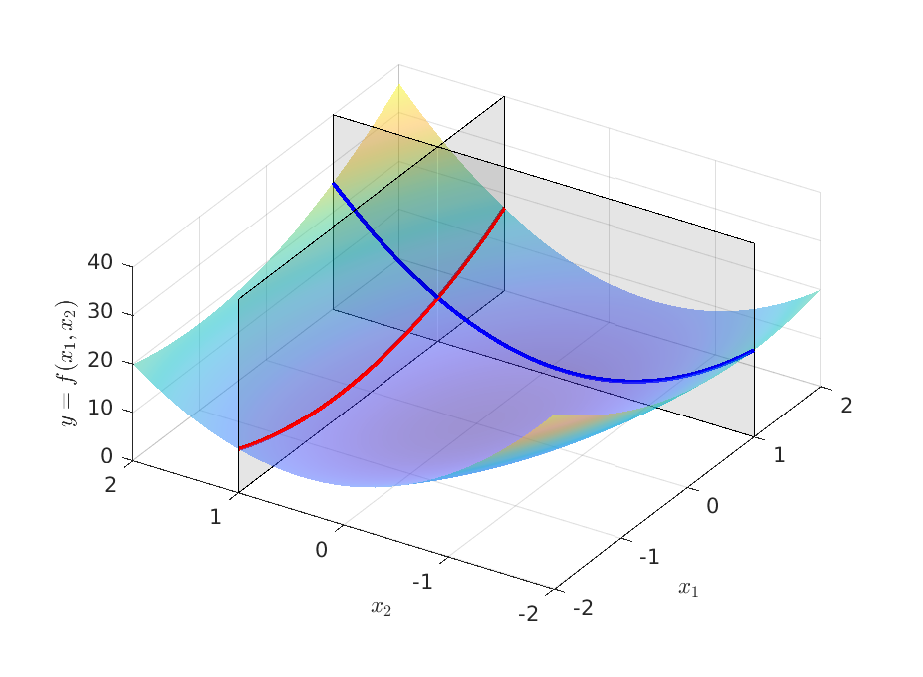
\includegraphics[width=250pt]{chapters/chapter6/figures/fig_motivatingexp.eps}
	\caption{Plot of function $y=f(x_1, x_2)$ in 3-D.} \label{ch6fig_motivatingexp}
\end{figure}

Let $x_2=1$ be constant. Equation \eqref{ch6eq:motivatingexample} becomes
\begin{eqnarray}
	y = f(x_1, 1) = 2x_1^2 + 2x_1 + 1, \nonumber
\end{eqnarray}
which is given by the intersection of  curved surface (equation \eqref{ch6eq:motivatingexample}) and the vertical flat ($x_2=1$) given by the red solid line in Fig. \ref{ch6fig_motivatingexp}. Its derivative with respect to $x_1$ can be easily obtained as
\begin{eqnarray}
	\dfrac{d}{dx_1}f(x_1,1) &=& 4x_1 + 2. \label{ch6eq:motivatingexpdx1}
\end{eqnarray}

Similarly, at $x_1 = 1$, \eqref{ch6eq:motivatingexample} becomes
\begin{eqnarray}
	y = f(1, x_2) = x_2^2 + 2x_2 + 2, \nonumber
\end{eqnarray}
which is given by the blue solid line in Fig. \ref{ch6fig_motivatingexp}. Its derivative with respect to $x_2$ is
\begin{eqnarray}
	\dfrac{d}{dx_2}f(1,x_2) &=& 2x_2 + 2. \label{ch6eq:motivatingexpdx2}
\end{eqnarray}

Consider small vibrations $\Delta x_1$ and $\Delta x_2$. Firstly, let $x_2$ remain constant and only apply $\Delta x_1$ on $y = f(1,1)$. In this case,
\begin{eqnarray}
	\Delta y = f(1+\Delta x_1, 1) - f(1, 1) \approx \dfrac{d}{dx_1}f(x_1,1) \Delta x_1, \label{ch6eq:partialdifx1}
\end{eqnarray}
where $\dfrac{d}{dx_1}f(x_1,1)$ is given in \eqref{ch6eq:motivatingexpdx1}.

On top of \eqref{ch6eq:partialdifx1}, consider vibration $\Delta x_2$. The derivative of function $f(1+\Delta x_1, x_2)$ with respect to $x_2$ depends on $\Delta x_1$ and it is generally unknown without specifying $\Delta x_1$. However, since \eqref{ch6eq:motivatingexample} is continuous and ``smooth'' (Notice that ``smooth'' has specific definition in mathematics. Here, just take its literal meaning: it is perfectly polished without any edges or spikes.), we can intuitively understand that when $\Delta x_1$ is small, $\frac{d}{dx_2}f(1+\Delta x_1, x_2) \approx \frac{d}{dx_2}f(1, x_2)$, and $\frac{d}{dx_2}f(1+\Delta x_1, x_2) \rightarrow \frac{d}{dx_2}f(1, x_2)$ as $\Delta x_1 \rightarrow 0$. Thus, we have
\begin{eqnarray}
	\Delta y &=& \left(f(1+\Delta x_1, 1 + \Delta x_2) -  f(1+\Delta x_1, 1)\right) + \left(f(1+\Delta x_1, 1) - f(1, 1)\right) \nonumber \\
	&\approx& \dfrac{d}{dx_2}f(1,x_2) \Delta x_2 + \dfrac{d}{dx_1}f(x_1,1) \Delta x_1. \label{ch6eq:motivatingresult1}
\end{eqnarray}

In \eqref{ch6eq:motivatingresult1}, consider $\Delta x_1 \rightarrow 0$ and $\Delta x_2 \rightarrow 0$. Denote such $\Delta x_1$ and $\Delta x_2$ as $dx_1$ and $dx_2$ respectively, and the associated $\Delta y$ as $dy$. Here ``$d(\cdot)$'' represents the \textit{infinitesimal change}. Equation \eqref{ch6eq:motivatingresult1} then becomes
\begin{eqnarray}
	d y &=& \dfrac{d}{dx_2}f(1,x_2) d x_2 + \dfrac{d}{dx_1}f(x_1,1) d x_1. \label{ch6eq:motivatingresult2}
\end{eqnarray}

Equation \eqref{ch6eq:motivatingresult2} can be extended to more general cases where $(x_1, x_2) = (1, 1)$ is not specified. The terms $\dfrac{d}{dx_1}f(x_1,1)$ and $\dfrac{d}{dx_2}f(1,x_2)$ needs to be changed accordingly. For example, $\dfrac{d}{dx_1}f(x_1,1)$ given by \eqref{ch6eq:motivatingexpdx1} shall be changed to
\begin{eqnarray}
	\left.\dfrac{d}{dx_1}f(x_1,x_2)\right|_{x_2 \textup{~is constant}} &=& 4x_1 + 2x_2 \nonumber
\end{eqnarray}
with $x_2$ being any arbitrary constant.

The denotation $\left.\dfrac{d}{dx_1}f(x_1,x_2)\right|_{x_2 \textup{~is constant}}$ can sometimes become ambiguous if not handled carefully. One of the reasons could be that ``$d(\cdot)$'' is used as infinitesimal change as shown before. In this case both $dx_1$ and $dx_2$ contribute to $df(x_1,x_2)$, but we would want $\dfrac{d}{dx_1}f(x_1,x_2)$ here to reflect the deviation of $f(x_1,x_2)$ caused by $dx_1$ only, and it is not convenient to list down all the other variables and put ``is/are constant'' everywhere in the equation. Therefore, instead of saying $\left.\dfrac{d}{dx_1}f(x_1,x_2)\right|_{x_2 \textup{~is constant}}$, we denote
\begin{eqnarray}
	\dfrac{\partial}{\partial x_1} f(x_1, x_2) &=& 4x_1 + 2x_2. \nonumber
\end{eqnarray}
The operator $\dfrac{\partial}{\partial x}$ is called \textit{partial derivative} (with respect to $x$), often followed by a multivariable function $f(x,y)$ where $x$ is one of its inputs. It is similar to the derivative, but emphasizing that the interested function is multivariable, and the derivative of this function with respect to ONLY ONE variable is being studied (and the rest variables assumed constant). Since $\partial f(x)$ is rarely or never used as the infinitesimal of $f(x)$, it will hopefully be less ambiguous.

The formal definition of partial derivative is given in next Section \ref{ch6sec:partialtotalderivative}.

Equation \eqref{ch6eq:motivatingresult2} for general $(x_1,x_2)$, therefore, becomes
\begin{eqnarray}
	d y &=& \dfrac{\partial}{\partial x_2}f(x_1,x_2) d x_2 + \dfrac{\partial}{\partial x_1}f(x_1,x_2) d x_1. \label{ch6eq:motivatingtotaldiff}
\end{eqnarray}

The minimum $y=f(x_1,x_2)$ and its associated $x_1$ and $x_2$ can be found by rewriting \eqref{ch6eq:motivatingexample} as
\begin{eqnarray}
	y &=& x_1^2 + \left(x_1 + x_2\right)^2. \nonumber
\end{eqnarray}
Therefore, the minimum $y$ is $y=0$, at $x_1 = 0$ and $x_1 + x_2 = 0$, i.e., $x_1 = x_2 = 0$.

This can also be solved using \eqref{ch6eq:motivatingtotaldiff}. At the minimum point of $y$, $\dfrac{\partial}{\partial x_2}f(x_1,x_2)$ and $\dfrac{\partial}{\partial x_1}f(x_1,x_2)$ must be both zero. Otherwise, it is always possible to add/subtract a small $\Delta x_1$ or $\Delta x_2$ to further decrease $y$. Thus, from \eqref{ch6eq:motivatingexample}
\begin{eqnarray}
	\dfrac{\partial}{\partial x_1}f(x_1,x_2) &=& 4x_1 + 2x_2 = 0 \nonumber \\
	\dfrac{\partial}{\partial x_2}f(x_1,x_2) &=& 2x_1 + 2x_1 = 0 \nonumber
\end{eqnarray}
which yields $x_1=x_2=0$.

\section{Partial Derivative} \label{ch6sec:partialtotalderivative}

In the case of single input scalar function $f(x), x \in \mathbb{R}$, there is no point to define partial and total derivative, as the derivative with respect to that single variable by itself is the total derivative.

In the case of multivariable function with multiple inputs, $f(x), x \in \mathbb{R}^{R\times 1}$, the definition partial derivative is given below.

\begin{VF}
	\textbf{Definition of Partial Integral}:
	\\
	\\
	Consider function $y = f(x_1,...,x_n)$ where $y$ is the scalar output and $x = \left[x_1, ..., x_n\right]^T$ is a $n\times 1$ vector input. The partial derivative of $y=f(x)$ with respect to $x_i$ is given by
	\begin{eqnarray}
		\dfrac{\partial}{\partial x_i}f(x) = \lim_{\Delta x_i \rightarrow 0} \dfrac{f(x_1,..., x_i + \Delta x_i,...,x_n)-f(x_1,...,x_n)}{\Delta x_i}, \label{ch6eq:formalpartialderivative}
	\end{eqnarray}
	with $x_1,...,x_{i-1}, x_{i+1},..., x_n$ remaining constant, and only $x_i$ is allowed to vary.
	
\end{VF}

Here is another example to help better understand partial derivative. Consider $z=f(x, y)$ a multivariable function of both inputs $x$, $y$ as follows
\begin{eqnarray}
	z = f(x,y) = x^2 + \textup{sin}(y), \label{ch6eq:partialdiffchainexp1}
\end{eqnarray}
where $y = g(x)$ is a single input function of $x$ as follows
\begin{eqnarray}
	y = g(x) = e^x. \label{ch6eq:partialdiffchainexp2}
\end{eqnarray}

Apparently, the value of $z$ ultimately depends on $x$ alone, but in the intermediate calculation, $z$ depends on both $x$ and $y$. The calculation flow is visualized in Fig. \ref{ch6fig_chainexp}.

\begin{figure}
	\centering
	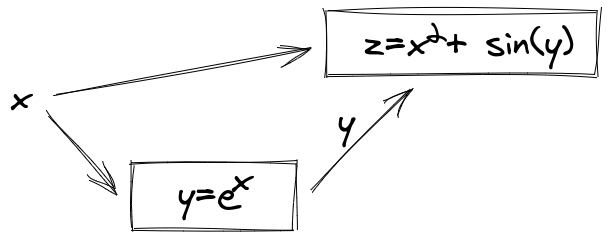
\includegraphics[width=200pt]{chapters/chapter6/figures/chainexp.png}
	\caption{The calculation of $z$ using $x$ and $y$.} \label{ch6fig_chainexp}
\end{figure}

In this case, the total derivative $\dfrac{d}{dx}f(x, y)$ can be expressed as follows
\begin{eqnarray}
	\dfrac{d}{dx}f(x, y) &=& \dfrac{\partial}{\partial x} f(x, y) + \dfrac{\partial}{\partial y}f(x, y) \dfrac{d}{dx}y. \label{ch6eq:partialvstotal}
\end{eqnarray}
where in this example,
\begin{eqnarray}
	\dfrac{\partial}{\partial x} f(x, y) &=& 2x \nonumber \\
	\dfrac{\partial}{\partial y} f(x, y) &=& \textup{cos}(y) \nonumber \\
	\dfrac{d}{dx}y &=& e^x \nonumber
\end{eqnarray}
and finally
\begin{eqnarray}
	\dfrac{d}{dx}f(x, y) &=& 2x + \textup{cos}(e^x)e^x \nonumber
\end{eqnarray}

Sometimes \eqref{ch6eq:partialvstotal} is rewritten as follows
\begin{eqnarray}
	df(x, y) &=& \dfrac{\partial}{\partial x} f(x, y) dx + \dfrac{\partial}{\partial y}f(x, y) dy \nonumber \\
	dy &=& \left(\dfrac{d}{dx}y\right) dx \nonumber
\end{eqnarray}
where $d(\cdot)$ represents the infinitesimal change of a variable.

Equation \eqref{ch6eq:partialvstotal} serves as a good example to show the relationship and difference between the total derivative $\dfrac{d}{dx}f(x, y)$ and the partial derivative $\dfrac{\partial}{\partial x} f(x, y)$. When calculating total derivative, all variables that would affect the value of the function must be taken into consideration, while when calculating partial derivative, only one input variable is studied, with the rest variables remaining constant.

For a function with $1$ output and $n$ inputs, sometimes it is convenient to put the partial derivative to each input in a vector. For example, for $y=f(x)$ where $x = \left[x_1,...,x_n\right]^T$, denote
\begin{eqnarray}
	\dfrac{\partial}{\partial x}f(x) = \left[\begin{array}{ccc}
	\dfrac{\partial}{\partial x_1}f(x) &
	\ldots &
	\dfrac{\partial}{\partial x_n}f(x)
	\end{array}\right] \label{ch6eq:scalarbyvector}
\end{eqnarray}
as the \textit{scalar-by-vector derivative}. Notice that \eqref{ch6eq:scalarbyvector} is usually given as a row vector. In some research papers the result is given as a column vector, i.e. the transpose of \eqref{ch6eq:scalarbyvector}.

For a function with $m$ outputs and $1$ input $y=f(x)$ where $y = \left[y_1,...,y_m\right]^T = \left[f_1(x),...,f_m(x)\right]^T$, its \textit{vector-by-scalar derivative} is given by
\begin{eqnarray}
	\dfrac{\partial}{\partial x}f(x) &=& \left[\begin{array}{c}
	\dfrac{\partial}{\partial x}f_1(x) \\
	\vdots \\
	\dfrac{\partial}{\partial x}f_m(x)
	\end{array}\right]. \label{ch6eq:vectorbyscalar}
\end{eqnarray}

And finally for a function with $m$ outputs and $n$ inputs $y=f(x)$ where $y = \left[y_1,...,y_m\right]^T = \left[f_1(x),...,f_m(x)\right]^T$ and $x = \left[x_1,...,x_n\right]^T$, the \textit{vector-by-vector} derivative is given by
\begin{eqnarray}
	\dfrac{\partial}{\partial x}f(x) &=& \left[\begin{array}{ccc}
	\dfrac{\partial}{\partial x_1}f_1(x) & \ldots & \dfrac{\partial}{\partial x_n}f_1(x) \\
	\vdots & \ddots & \vdots \\
	\dfrac{\partial}{\partial x_1}f_m(x) & \ldots & \dfrac{\partial}{\partial x_n}f_m(x) \\
	\end{array}\right]. \label{ch6eq:vectorbyvector}
\end{eqnarray}

Partial derivative and the above equations \eqref{ch6eq:scalarbyvector}, \eqref{ch6eq:vectorbyscalar} and \eqref{ch6eq:vectorbyvector} have many applications. Two of those most popular use cases are \textit{gradient} and \textit{Jacobian matrix}. Since they are so important and widely used, it is worth especially introducing them in specific Sections \ref{ch6sec:gradient} and \ref{ch6sec:jacobianmatrix}.

\section{Gradient} \label{ch6sec:gradient}

For a scalar-valued multivariable function $y=f(x)$ where $y$ is a scalar and $x$ is a vector $x = \left[\begin{array}{ccc}
                                                                               x_1 & \ldots & x_n
                                                                             \end{array}\right] \in \mathbb{R}^n$, the gradient studies the ``direction'' of $\Delta x$ in $\mathbb{R}^n$ space that causes $y$ to increase/decrease the fastest.

The gradient of such function $f(x)$ is a vector function of $x$, denoted by $\nabla f(x)$. Notice that $\nabla f(x) \in \mathbb{R}^n$ is a vector in the same space with $x$, since it indicates a ``direction'' of $x$.

Section \ref{ch6subsec:gradientmotivatingexp} gives a motivating example of gradient, and Section \ref{ch6subsec:gradientdef} gives its formal definition.

\subsection{Motivating Example} \label{ch6subsec:gradientmotivatingexp}

The following motivating example helps to illustrate the calculation and use case of gradient.

\begin{shortbox}
\Boxhead{A Motivating Example}

Consider the following function $y=f(x_1,x_2)$
\begin{eqnarray}
    y = f(x_1,x_2) = 2\textup{sin}(x_1) + \textup{sin}\left(\dfrac{x_1}{2} + \pi\right) + \textup{sin}(2x_2) \label{ch6eq:gradientexp_hill}
\end{eqnarray}
where $x_1\in[-3,3]$ and $x_2\in[-2,2]$. The 3-D plot and the contour line of the function are given in Figs \ref{ch6fig:gradientexp_3d} and \ref{ch6fig:gradientexp_contour} respectively.

The objective is to obtain such $x_1$ and $x_2$ to maximize $y$. By applying a glomal optimization on \eqref{ch6eq:gradientexp_hill}, $x_1 = 1.3764$, $x_2=0.7854$ can be obtained. However, in this example we are assuming that the global optimization is not applicable due to the lack of information or computational power. Try to obtain the target coordinate $x_1$ and $x_2$ without using global optimization.

\end{shortbox}

\begin{figure}
	\centering
	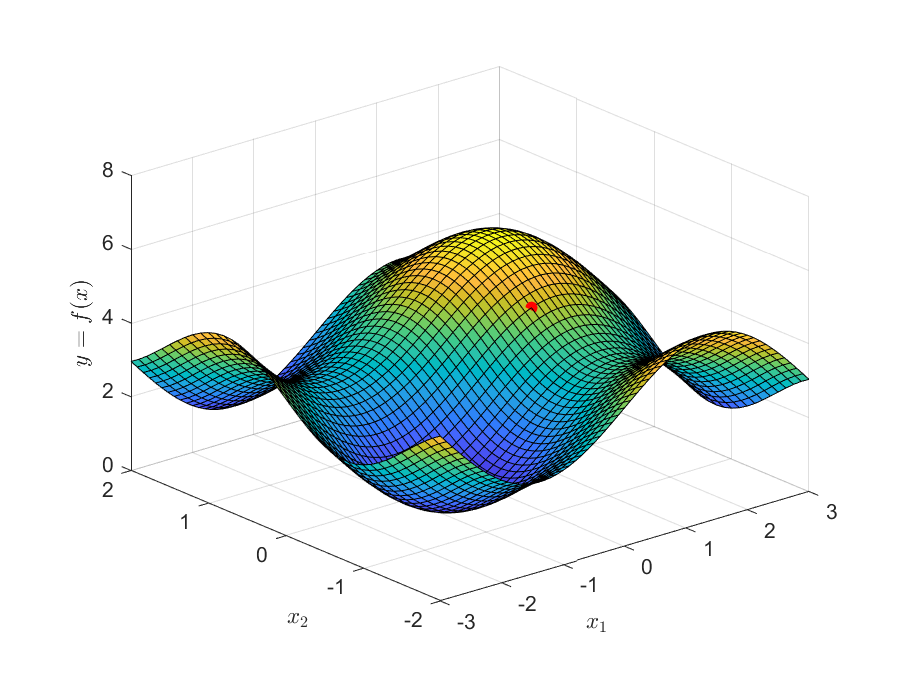
\includegraphics[width=250pt]{chapters/chapter6/figures/gradientexp_3d.eps}
	\caption{Plot of $y=f(x_1, x_2)$ in 3-D.} \label{ch6fig:gradientexp_3d}
\end{figure}
\begin{figure}
	\centering
	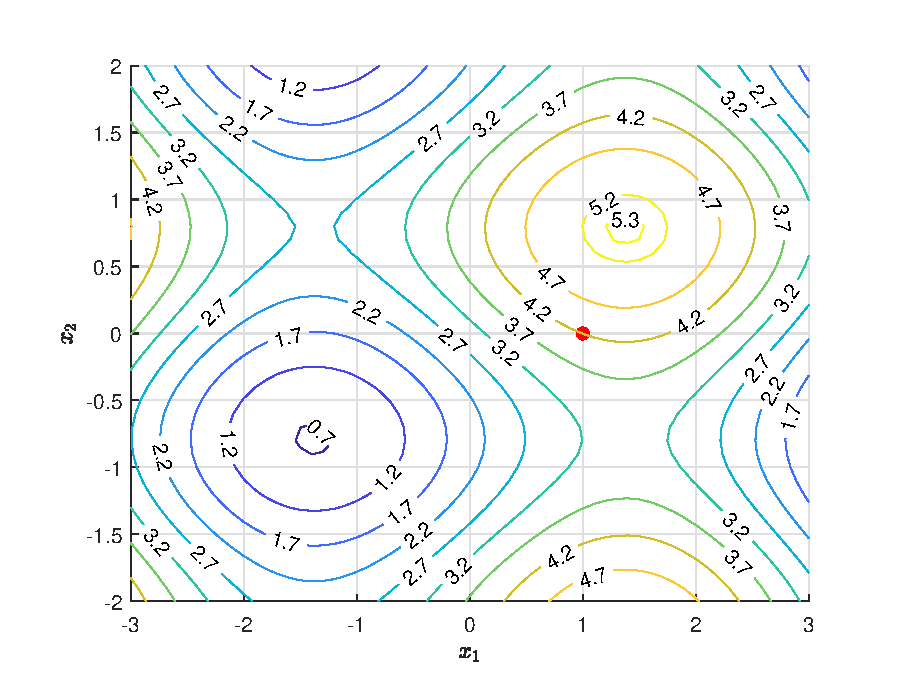
\includegraphics[width=250pt]{chapters/chapter6/figures/gradientexp_contour.eps}
	\caption{Contour line of $y=f(x_1, x_2)$.} \label{ch6fig:gradientexp_contour}
\end{figure}

We are using iterations to find the maximum point of $y$ and associated $x_1$ and $x_2$ as follows.

Step 1: Start at initial point $x^0 = [1,0]$, which is marked by a red dot on both Figs. \ref{ch6fig:gradientexp_3d} and \ref{ch6fig:gradientexp_contour}.

Step 2: Determine a small change $\Delta x^k = [\Delta x_1^k, \Delta x_2^k]$. Such $[\Delta x_1^k, \Delta x_2^k]$ shall maximize $f(x_1^k+\Delta x_1^k, x_2^k+\Delta x_2^k)$ as much as possible, without introducing too much computational complexity.

Step 3: Let $x^{k+1} = x^k + \Delta x^k$.

Steps 2 and 3 are executed recursively until $f(x_1^{k+1}, x_2^{k+1}) \approx f(x_1^k, x_2^k)$. In this way, hopefully $x^k$ can slowly ``climb up'' to the maximum point of $y$ in Fig. \ref{ch6fig:gradientexp_3d}.

The remaining problem is how to find $\Delta x^k = [\Delta x_1^k, \Delta x_2^k]$ in Step 2 to best maximize $f(x_1^k+\Delta x_1^k, x_2^k+\Delta x_2^k)$ with minimum information and calculation load.

Notice that $\Delta x^k$ can be interpreted as a vector that indicates the ``direction'', along which trace the value of $y$ increases the fastest. An intuitive way is to find the tangent plane to the surface. From space analytic geometry, we know that a pair of unparalleled vector can uniquely define a plane, and such pair of vector is not difficult to find, as
\begin{eqnarray}
 \vec{v}_1 &=& \left(1,0,\left.\dfrac{\partial y}{\partial x_1}\right|_{x=x^k}\right) \label{ch6eq:gradientexp_v1} \\
 \vec{v}_2 &=& \left(0,1,\left.\dfrac{\partial y}{\partial x_2}\right|_{x=x^k}\right) \label{ch6eq:gradientexp_v2}
\end{eqnarray}
must be such a pair of vector. This is because \eqref{ch6eq:gradientexp_v1} is the tangent of the 2-D intersect of $y=f(x_1,x_2)$ and $x_2 = x_2^k$ (i.e. $y=f(x_1,x_2^k)$), therefore must be tangent to the original 3-D surface $y=f(x_1,x_2)$. The same applies to \eqref{ch6eq:gradientexp_v2}, making it also tangent to $y=f(x_1,x_2)$. And obviously the two lines are unparalleled since one of them lies on plane $x_1=x_1^k$ and the other on plane $x_2=x_2^k$, which are two perpendicular planes.

Take the $x^k=x^0=[1,0]$ as an example. The intersect of $y=f(x_1,x_2)$ and $x_2 = 0$ is given as the red solid line in Fig. \ref{ch6fig:gradientexp_3d2}, and its tangent at $\left(1,0,f(1,0)\right)$, i.e. equation \eqref{ch6eq:gradientexp_v1}, is given by the red dashed line. The same is applied for the intersect of $y=f(x_1,x_2)$ and $x_1 = 1$ and its tangent equation \eqref{ch6eq:gradientexp_v2} as the blue lines.

\begin{figure}
	\centering
	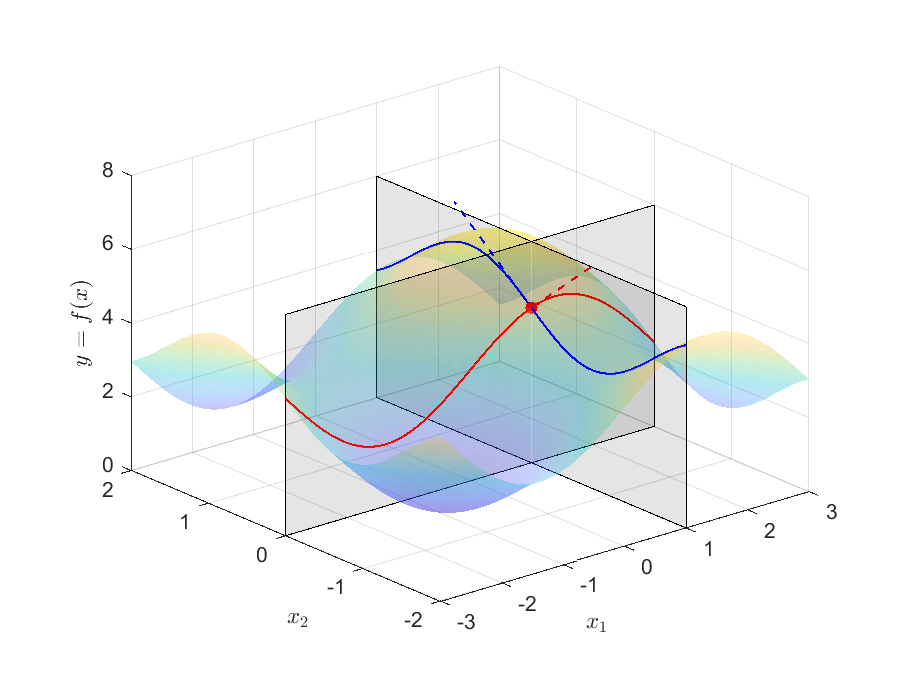
\includegraphics[width=250pt]{chapters/chapter6/figures/gradientexp_3d2.eps}
	\caption{Plot of vectors given by \eqref{ch6eq:gradientexp_v1} and \eqref{ch6eq:gradientexp_v2}.} \label{ch6fig:gradientexp_3d2}
\end{figure}

The two vectors \eqref{ch6eq:gradientexp_v1} and \eqref{ch6eq:gradientexp_v2}, as indicated by the red and blue dashed lines respectively in Fig. \ref{ch6fig:gradientexp_3d2} are unparalleled and intersect at $\left(1,0,f(1,0)\right)$. Therefore, the vectors can uniquely determine a plane which is the tangent plan for $y=f(x_1,x_2)$ at $\left(1,0,f(1,0)\right)$, as shown by Fig. \ref{ch6fig:gradientexp_3d3}.

\begin{figure}
	\centering
	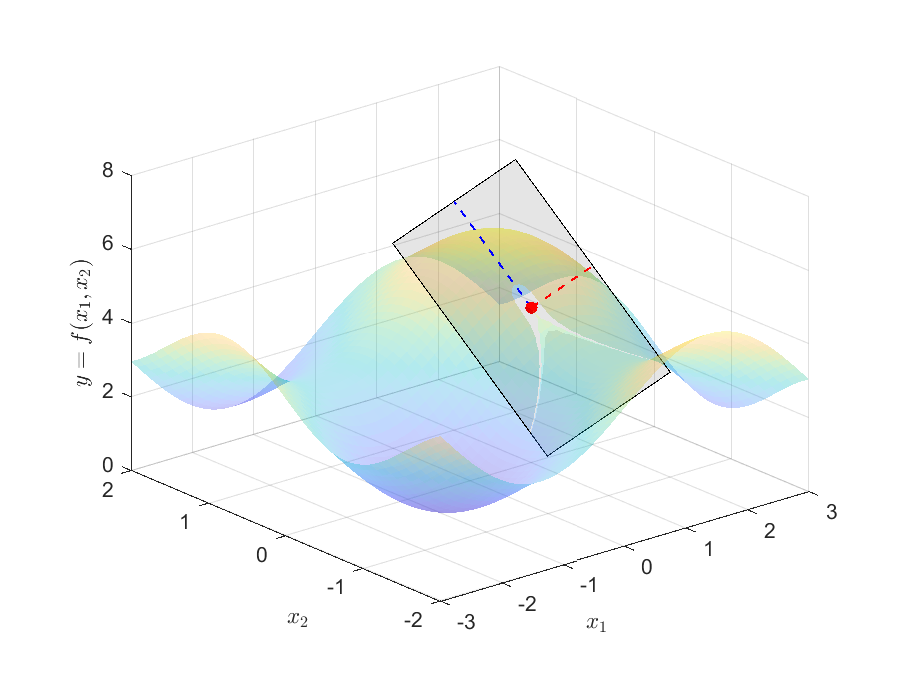
\includegraphics[width=250pt]{chapters/chapter6/figures/gradientexp_3d3.eps}
	\caption{Formulation of the tangent plane from vectors given by \eqref{ch6eq:gradientexp_v1} and \eqref{ch6eq:gradientexp_v2}.} \label{ch6fig:gradientexp_3d3}
\end{figure}

The next step is to find a vector on the tangent plane along which $y$ increases the fastest. The direction of this vector will be used as a guidance in selecting $\Delta x^k = [\Delta x_1^k, \Delta x_2^k]$. This vector can be derived using space analytic geometry and it is briefly introduced as follows. 

For such a vector, it must fulfill the following two conditions: (a) it must be on the tangent plane; (b) it must be perpendicular to the intersection line of the tangent plane and the $y=0$ plane.

Consider (a). Since the vector is on the tangent plan, it can be represented as a linear combination of \eqref{ch6eq:gradientexp_v1} and \eqref{ch6eq:gradientexp_v2} as
\begin{eqnarray}
    && \left(\lambda_1, \lambda_2, \lambda_1\left.\dfrac{\partial y}{\partial x_1}\right|_{x=x^k} + \lambda_2\left.\dfrac{\partial y}{\partial x_2}\right|_{x=x^k} \right) . \nonumber
\end{eqnarray}

Consider (b). The analytical expression for the tangent plane can be obtained by calculating its normal vector as follows.
\begin{eqnarray}
  \vec{n} &=& \vec{v}_1 \times \vec{v}_2
\end{eqnarray}














\subsection{Gradient of a Multivariable Function} \label{ch6subsec:gradientdef}




\section{Jacobian Matrix} \label{ch6sec:jacobianmatrix}
